\documentclass[pdflatex, 12pt]{beamer}
\usetheme{Boadilla}
\usefonttheme{professionalfonts}

\usepackage{graphicx}
\usepackage{color}
\usepackage{amsmath, amssymb}
\usepackage{bm}
%\usepackage{enumitem}
\usepackage{natbib}
\usepackage{url}
\usepackage{wasysym}
\usepackage{setspace}
\usepackage{tikz}

%\setbeamerfont{title}{series=\bfseries}
%\setbeamerfont{frametitle}{series=\bfseries}

%\setbeamercolor{title}{fg=violet}
%\setbeamercolor{frametitle}{fg=violet}

%\setbeamercolor{palette primary}{fg=black, bg=violet!50}
%\setbeamercolor{palette secondary}{fg=violet, bg=white}
%\setbeamercolor{palette tertiary}{fg=black, bg=violet!70}

\setbeamertemplate{navigation symbols}{}

%\setbeamertemplate{itemize item}{\color{violet}$\bullet$}
%\setbeamertemplate{itemize subitem}{\color{violet}\scriptsize{$\blacktriangleright$}}
%\setbeamertemplate{itemize subsubitem}{\color{violet}$\star$}

\setbeamertemplate{itemize item}{$\bullet$}
\setbeamertemplate{itemize subitem}{\scriptsize{$\blacktriangleright$}}
\setbeamertemplate{itemize subsubitem}{$\star$}

\setbeamertemplate{enumerate items}[default]

\newcommand{\R}{\mathbb{R}}
\newcommand{\Q}{\mathbb{Q}}
\newcommand{\Z}{\mathbb{Z}}
\newcommand{\N}{\mathbb{N}}

\title[Math Camp: Day 5]{Day 5: Probability}
\author[Ikuma Ogura]{Ikuma Ogura}
\institute[Georgetown]{Ph.D. student, Department of Government, Georgetown University}
\date[August 23, 2019]{August 23, 2019}

\begin{document}

\begin{frame}
\frametitle{}
\titlepage
\end{frame}

\begin{frame}
\frametitle{Today}
\begin{itemize}
\item Today
 \begin{itemize}
 \item Probability
 \item Random variable
 \item Probability distribution
 \item (if time permits) Probability distributions in R
 \end{itemize}
\end{itemize}
\end{frame}

\begin{frame}
\frametitle{Why Probability?}
\begin{itemize}
\item Foundation of statistical inference
\vspace{0.4cm}
\item Formal modeling/game theory: describe uncertainty
\end{itemize}
\end{frame}

\begin{frame}
\frametitle{Probability and Statistics}
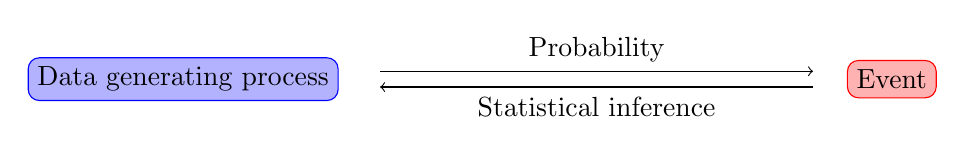
\begin{tikzpicture}
\node[draw = blue, fill = blue!30, rounded corners] (X) at (0,0) {Data generating process};
\node[draw = red, fill = red!30, rounded corners] (Y) at (9, 0) {Event};
\draw[->] (2.5, 0.1) -- (8, 0.1) node[midway, above] {Probability};
\draw[->] (8, -0.1) -- (2.5, -0.1) node[midway, below] {Statistical inference};
\end{tikzpicture}
\vspace{0.4cm}
\begin{itemize}
\item Probability: explains how likely each event occurs based on the known data generating process (DGP)
\vspace{0.4cm}
\item Statistical inference: infer the DGP based on the data (= collection of events)
\end{itemize}
\end{frame}

\begin{frame}
\frametitle{Probability}
\begin{itemize}
\item \textbf{Sample space} ($S$): A set/collection of all possible outcomes from some process. 
 \begin{itemize}
 \item Outcomes of sample space can be countable (discrete) or uncountable (continuous).
 \end{itemize}
\vspace{0.4cm}
\item \textbf{Event}: Any set of possible outcomes from the process. Any subset of the full set of possibilities (= sample space), including the full set itself.
\vspace{0.4cm}
\item \textbf{Partition}: a sequence of disjoint events $A_1, A_2, \cdots, A_n$ where
 \begin{equation}
 A_1 \cup A_2 \cup \cdots \cup A_n = S \notag
 \end{equation}
\end{itemize}
\end{frame}

\begin{frame}
\frametitle{Probability (cont.)}
\begin{itemize}
\item \textbf{Probability} is a function that maps events to a real number and follows the \textbf{axioms of probability} below.
 \begin{enumerate}
 \item For any event $A$, $\Pr(A) \geq 0$.
 \item $\Pr(S) = 1$.
 \item For any sequence of disjoint events $A_1, A_2, \cdots$
  \begin{equation}
  \Pr(A_1 \cup A_2 \cup \cdots ) = \Pr(\bigcup_{i = 1} A_i) = \sum_{i = 1} \Pr(A_i) \notag
  \end{equation}
 \end{enumerate}
\end{itemize}
\end{frame}

\begin{frame}
\frametitle{Probability (cont.)}
\begin{itemize}
\item Example 1: Let $A_i$ denote the event of getting hand $i$ in the game of poker. Then, probability of hand $i$ can be defined as 
 \begin{equation}
 \Pr(A_i) = \frac{\mathrm{Frequency \ of\ getting \ hand \ }i}{\mathrm{Number \ of\ all \ possible \ outcomes}} \notag
 \end{equation}
\end{itemize}
\end{frame}

\begin{frame}
\frametitle{Probability (cont.)}
\begin{columns}
\begin{column}{0.5\textwidth}
\centering
\includegraphics[scale = 0.17]{fig5_1.png}
\end{column}
\begin{column}{0.5\textwidth}
\begin{itemize}
\item Example 2: Ikuma is novice in archery. Assuming that he can always hit the target (!), what is the probability of scoring point $i$?
\vspace{0.4cm}
\item Let $A_i$ denote the event of scoring $i$, 
 \begin{equation}
 \Pr(A_i) = \frac{\mathrm{Area \ of \ region\ }i}{\mathrm{Total \ area}} \notag
 \end{equation}
\end{itemize}
\end{column}
\end{columns}
\end{frame}

\begin{frame}
\frametitle{Probability (cont.)}
\begin{itemize}
\item Properties of probability operation
 \begin{enumerate}
 \item $\Pr(\emptyset) = 0.$
 \item $0 \leq \Pr(A) \leq 1$
 \item $\Pr(A^c) = 1 - \Pr(A)$
 \item If $A \subseteq B$, $\Pr(A) \leq \Pr(B)$
 \end{enumerate}
\end{itemize}
\end{frame}

\begin{frame}
\frametitle{Counting}
\begin{itemize}
\item Counting \textit{with replacement} or \textit{without replacement}
\vspace{0.4cm}
\item \textit{Ordering} is important or not
\vspace{0.4cm}
\item Below let's think of a case in which we select $k$ out of $n$.
\end{itemize}
\end{frame}

\begin{frame}
\frametitle{Counting (cont.)}
\begin{itemize}
\item \textbf{Ordered, with replament}: in this case, the number of different outcomes is
 \begin{equation}
 n^k \notag
 \end{equation}
\vspace{0.2cm}
\item \textbf{Ordered, without replament}: in this case the number of different outcomes is
 \begin{equation}
 n \times (n - 1) \times (n - 2) \times \cdots \times (n - k + 1) = \frac{n!}{(n - k)!} \notag
 \end{equation}
\end{itemize}
\end{frame}

\begin{frame}
\frametitle{Counting (cont.)}
\begin{itemize}
\item \textbf{Unordered, without replament}: as there is $k!$ ways to order $k$ objects, the number of different outcomes in this case is
 \begin{equation}
 \frac{n \times (n - 1) \times (n - 2) \times \cdots \times (n - k + 1)}{k!} = \frac{n!}{k!(n - k)!} = \binom{n}{k} \notag
 \end{equation}
 \begin{itemize}
 \item $\binom{n}{k}$ is called the binomial coefficient
 \end{itemize}
\end{itemize}
\end{frame}

\begin{frame}
\frametitle{Counting (cont.)}
\begin{itemize}
\item Example: What is the probability of getting full house? 
 \begin{itemize}
 \item Denominator: the number different ways to select 5 cards out of 52 is $\binom{52}{5}$.
 \item Numerator: we need to choose 3 cards from one face value, and 2 cards from another face value. Therefore, the number of distinct hands is
  \begin{equation}
  \binom{13}{1} \binom{4}{3} \binom{12}{1} \binom{4}{2} \notag
  \end{equation}
 \item Therefore, the probability of getting full house is
  \begin{equation}
  \frac{13 \cdot 4 \cdot 12 \cdot 6}{\frac{52 \cdot 51 \cdot 50 \cdot 49 \cdot 48}{5 \cdot 4 \cdot 3 \cdot 2 \cdot 1}} = \frac{6}{4165} \approx 0.00144 \notag
  \end{equation}
 \end{itemize}
\end{itemize}
\end{frame}

\begin{frame}
\frametitle{Counting: Exercises}
\begin{enumerate}
\item (de Mere's problem) Which is higher:
 \begin{enumerate}
 \item the probability of getting at least one ``6'' in 4 rolls of a 6-sided die
 \item the probability of at least one double-six in 24 rolls of two dice
 \end{enumerate}
\vspace{0.4cm}
\item (Birthday problem) Suppose 20 individuals are randomly selected. Find the probability that at least two of them have the same birthday. 	
\end{enumerate}
\end{frame}

\begin{frame}
\frametitle{Counting: Exercises (cont.)}
\begin{itemize}
\item Calculate the probability of the following in the game of poker.
 \begin{enumerate}
 \item One pair
 \item Two pair
 \item Three of a kind
 \item Straight (excluding straight flush)
 \item Flush (excluding straight flush)
 \item Straight flush
 \item Four of a kind
 \item No pair
 \end{enumerate}
\end{itemize}
\end{frame}

\begin{frame}
\frametitle{Conditional Probability}
\begin{itemize}
\item \textbf{Conditional probability} $\Pr{A|B}$ is the probability of event $A$ given that the event $B$ occurred, which is defined as 
 \begin{equation}
 \Pr(A|B) = \frac{\Pr(A \cap B)}{\Pr(B)} \notag
 \end{equation}
\vspace{0.2cm}
\item If $\Pr(A) \neq 0$, $\Pr(A \cap B) = \Pr(A|B)\Pr(B)$
\vspace{0.4cm}
\item If $\Pr(A|B) = \Pr(A)$, events $A$ and $B$ are said to be \textbf{independent}.
 \begin{itemize}
 \item Equivalently, if $A$ and $B$ are independent,s $\Pr(A \cap B) = \Pr(A)\Pr(B)$
 \end{itemize}
\end{itemize}
\end{frame}

\begin{frame}
\frametitle{Conditional Probability (cont.)}
\begin{itemize}
\item Example: what is the probability of choosing the Ace of heart given that the selected card is red? Let
 \begin{eqnarray}
 A &=& \left\{\mathrm{Choose \ Ace \ of \ Heart}\right\} \notag \\
 R &=& \left\{\mathrm{Choose \ Red}\right\}, \notag
 \end{eqnarray}
the probability of interest is 
 \begin{equation}
 \Pr(A|R) = \frac{\Pr(A \cap R)}{\Pr(R)} = \frac{\Pr(A)}{\Pr(R)} = \frac{1}{26} \notag
 \end{equation}
\end{itemize}
\end{frame}

\begin{frame}
\frametitle{Bayes Rule}
\begin{itemize}
\item \textbf{Law of Total Probability}: Let $B_1, B_2, \cdots, B_n$ be the partition of $S$. For some event $A$ in $S$, we can represented the set as the union of disjoint subsets 
 \begin{equation}
 A = (A \cap B_1) \cup (A \cap B_2) \cup \cdots \cup (A \cap B_n). \notag
 \end{equation}
Therefore, from the axiom of probability,
 {\small
 \begin{equation}
 \Pr(A) = \Pr(A \cap B_1) + \Pr(A \cap B_2) + \cdots + \Pr(A \cap B_n) = \sum_{i = 1}^{n} \Pr(A \cap B_i) \notag
 \end{equation}
 }
\end{itemize}
\end{frame}

\begin{frame}
\frametitle{Bayes Rule (cont.)}
\begin{itemize}
\item Example: the probability of choosing a heart is 
 \begin{eqnarray}
 \Pr(\mathrm{Choose \ Heart}) &=& \Pr(\mathrm{Choose \ Heart} \cap \mathrm{Choose \ A}) + \notag \\
 &=& \Pr(\mathrm{Choose \ Heart} \cap \mathrm{Choose}\ 2) + \notag \\
 &=& \cdots + \notag \\
 &=& \Pr(\mathrm{Choose \ Heart} \cap \mathrm{Choose \ King}) \notag 
 \end{eqnarray}
\end{itemize}
\end{frame}

\begin{frame}
\frametitle{Bayes Rule (cont.)}
\begin{itemize}
\item \textbf{Bayes rule}: Let $B_1, B_2, \cdots, B_n$ be the partition of $S$. Based on the defition of conditional probability and the law of total probability, 
 \begin{equation}
 \Pr(B_k|A) = \frac{\Pr(A \cap B_k)}{\Pr(A)} = \frac{\Pr(A|B_k)\Pr(B_k)}{\sum_{i = 1}^{n} \Pr(A|B_i)\Pr(B_i)} \notag
 \end{equation}
 \begin{itemize}
 \item $\Pr(B_k)$ is called the prior probability.
 \item Bayes rule describes how $\Pr(B_k)$ changes with additional information.
 \end{itemize}
\end{itemize}
\end{frame}

\begin{frame}
\frametitle{Bayes Rule: Example}
\begin{itemize}
\item Example: (Monty Hall problem) You are on a game show and asked to choose between three doors. Behind each door, there is either a car or a goat. After you choose a door, the host, Monty, opens another door, shows a goat, and gives you a chance to change your choice. Should you change your choice?
\vspace{0.4cm}
 \begin{itemize}
 \item Answer: let's name the three doors A, B, and C, and represent the event that a car is behind the corresponding door. Let $X_{M} \ (X \in \left\{A, B, C\right\})$ denote the event that Monty opens the door $X$. For generality, let's assume you pick the door $A$ and Monty opens the door $B$. Therefore, we need to compare the probability $\Pr(A|B_{M})$ and $\Pr(C|B_{M})$. Here, let's also assume that
  \begin{equation}
  \Pr(A) = \Pr(B) = \Pr(C) = \frac{1}{3}. \notag
  \end{equation}  
 \end{itemize}
\end{itemize}
\end{frame}

\begin{frame}
(\emph{continue from the previous slide})

\vspace{0.4cm}
Applying the Bayes rule,
{\footnotesize
\begin{eqnarray}
\Pr(A|B_{M}) &=& \frac{\Pr(B_M|A)\Pr(A)}{\Pr(B_M|A)\Pr(A) + \Pr(B_M|B)\Pr(B) + \Pr(B_M|C)\Pr(C)} \notag \\
&=& \frac{\frac{1}{2} \cdot \frac{1}{3}}{\frac{1}{2} \cdot \frac{1}{3} + 0 + 1 \cdot \frac{1}{3}} = \frac{1}{3} \notag
\end{eqnarray}
}
and 
{\footnotesize
\begin{eqnarray}
\Pr(C|B_{M}) &=& \frac{\Pr(B_M|C)\Pr(C)}{\Pr(B_M|A)\Pr(A) + \Pr(B_M|B)\Pr(B) + \Pr(B_M|C)\Pr(C)} \notag \\
&=& \frac{1 \cdot \frac{1}{3}}{\frac{1}{2} \cdot \frac{1}{3} + 0 + 1 \cdot \frac{1}{3}} = \frac{2}{3} \notag
\end{eqnarray}
}
Therefore, you should switch the door you choose from $A$ to $C$.
\end{frame}

\begin{frame}
\frametitle{Bayes Rule: Exercise}
\begin{itemize}
\item In Orange County, 51\% of the adults are men. One adult is randomely selected for a survey, and the selected survey subjest was smoking cigarettes. Based on administrative data, we know that 16\% of men smoke cigarettes, whereas 12\% of women do so. What is the probability that the selected subject is a man?
\end{itemize}
\end{frame}

\begin{frame}
\frametitle{Random Variable}
\begin{itemize}
\item \textbf{Random variable} is a function from a sample space to real numbers.
\vspace{0.4cm}
\item We use capital letters (e.g., $X$) to represent random variables and small letters (e.g., $x$) to denote their realizations (concrete values they take).
\vspace{0.4cm}
\item We can also define probability for a random variable.
 \begin{equation}
 \Pr(X = x_i) = \Pr(\left\{s_j \in S|X(s_j) = x_i\right\}) \notag
 \end{equation}
\item Discrete v. Continuous 
 \begin{itemize}
 \item A random variable $X$ is \textbf{discrete} if it takes finite or countably infinite number of values
 \item A random variable $X$ is \textbf{continuous} if it can take any real numbers in the domain
 \item continuous sample space does not nessarily lead to contious random varialbe (see example)
 \end{itemize}
\end{itemize}
\end{frame}

\begin{frame}
\frametitle{Random Variable (cont.)}
\begin{itemize}
\item Example 1: we can assign scores to poker hands as follows:
 \begin{table}
 \scalebox{0.9}{
 \begin{tabular}{l l }
 \hline\hline
 Hand & Score ($X$) \\\hline
 No pair & $0$ \\
 One pair & $1$ \\
 Two pair & $2$ \\
 Three of a kind & $3$ \\
 Straight & $4$ \\
 Flush & $5$ \\
 Full house & $6$ \\
 Four of a kind & $7$ \\
 Straight flush & $8$ \\\hline
 \end{tabular}
 }
 \end{table}
Here, outcomes in the sample space (= combination of 5 cards) are mapped to real numbers (score $X$).
\end{itemize} 
\end{frame}

\begin{frame}
\frametitle{Random Variable (cont.)}
\begin{itemize}
\item Example 2: For the example of archery we saw earlier, we can define the random variable $X$ as 
 \begin{equation}
 X(\left\{\mathrm{Arrow \ hits \ the \ region \ }i\right\}) = i. \notag
 \end{equation}
In this case, even though the sample space is continuous, the random variable $X$ is discrete.
\end{itemize}
\end{frame}

\begin{frame}
\frametitle{Random Variable (cont.)}
\begin{itemize}
\item Example 3: Define the random variable $T$ to denote the time until the next train arrives at the station. Here, $T$ is a continuous random variable since it can take any real numbers.
\end{itemize}
\end{frame}

\begin{frame}
\frametitle{Random Variable (cont.)}
\begin{itemize}
\item Randomness does not mean lack of pattern/structure/order.
 \begin{itemize}
 \item Randomness means that the outcome of some process/realization of the variable is not deterministic.
 \item Pattern/structure/order of the process is characterized by probability.
 \end{itemize}
\end{itemize}
\end{frame}

\begin{frame}
\frametitle{Probability Distribution}
\begin{itemize}
\item Probability distributions specify the relationship between the random variable and probabilities.
\vspace{0.4cm}
\item Below I'll introduce two types of functions describing a probability distribution.  
\end{itemize}
\end{frame}

\begin{frame}
\frametitle{Probability Mass/Density Function}
\begin{itemize}
\item \textbf{Probability mass function (PMF)} for a discrete random variable $X$ describes the probability that $X$ takes a specific value $x$.
 \begin{equation}
 f(x) = \Pr(X = x) \notag
 \end{equation}
\vspace{0.4cm}
\item We can also consider similar function $f(x)$ for a continuous random variable $X$, which is called the \textbf{probability density function (PDF)}.   
\end{itemize}
\end{frame}

\begin{frame}
\frametitle{Probability Mass/Density Function (cont.)}
\begin{itemize}
\item Example: Let $X$ be the sum of numbers we get by rolling two dice. Assuming that these dice are fair, the PMF $f(x)$ is
 \begin{equation}
 f(x) = \Pr(X = x) = \frac{6 - |7 - x|}{36} \notag
 \end{equation}
\end{itemize}
\end{frame}

\begin{frame}
\frametitle{Probability Mass/Density Function (cont.)}
\begin{columns}
\begin{column}{0.5\textwidth}
\includegraphics[scale = 0.6]{fig5_2.pdf}
\end{column}
\begin{column}{0.5\textwidth}
\begin{itemize}
\item For a continuous random variable, we cannot allow a point $X = x$ to have probability larger than 0!
\vspace{0.4cm}
\item $f(x)$ describes the \emph{relative likelihood} that $X$ equals to $x$.
\vspace{0.4cm}
\item Instead, for a continuous distribution we define probability for an interval in the domain.
\end{itemize}
\end{column}
\end{columns}
\end{frame}

\begin{frame}
\frametitle{Probability Mass/Density Function (cont.)}
\begin{columns}
\begin{column}{0.5\textwidth}
\includegraphics[scale = 0.6]{fig5_3.pdf}
\end{column}
\begin{column}{0.5\textwidth}
\begin{itemize}
\item The probability of $X$ falling between $(a, b)$ equal to
 \begin{equation}
 \Pr(a < x < b) = \int^b_a f(x) dx \notag
 \end{equation}
\vspace{0.2cm}
\item As the probability of a single point is 0, 
 {\small
 \begin{equation}
 \Pr(a < x < b) = \Pr(a \leq x \leq b) \notag 
 \end{equation}
 }
\end{itemize}
\end{column}
\end{columns}
\end{frame}

\begin{frame}
\frametitle{Cumulative Density Function}
\begin{itemize}
\item \textbf{Cumulative density function} (CDF) describes the probability that the random variable $X$ is smaller than or euqal to $x$.
 \begin{itemize}
 \item For a discrete random variable, CDF is defined as 
  \begin{equation}
  F(x) = \Pr(X \leq x) = \sum_{i \leq x} f(i) \notag
  \end{equation}
 \item For a continuous random variable, CDF is defined as 
  \begin{equation}
  F(x) = \Pr(X \leq x) = \int^x_{-\infty} f(t) dt \notag
  \end{equation}
 \end{itemize}
\end{itemize}
\end{frame}

\begin{frame}
\frametitle{Cumulative Density Function (cont.)}
\begin{itemize}
\item For a continuous random variable, from the fundamental theorem of calculus, 
 \begin{equation}
 F'(x) = f(x) \notag
 \end{equation}
\vspace{0.2cm}
\item CDF of a discrete distribution is a step function, whereas CDF of a continuous distribution is a continuous function.
\vspace{0.4cm}
\item Properties of CDF
 \begin{enumerate}
 \item $F(x)$ is a non-decreasing function of $x$
 \item $\lim_{x \to -\infty} F(x) = 0$ and $\lim_{x \to \infty} F(x) = 1$
 \item $F(x)$ is right-continuous, meaning that, for every $x_0$ in the domain $\lim_{x \to x_0^{+}} F(x) = F(x_0)$
 \end{enumerate}
\end{itemize}
\end{frame}

\begin{frame}
\frametitle{Cumulative Density Function: Exercise}
\begin{itemize}
\item Draw the CDF of the random variable for sum of two dice we saw earlier.
\end{itemize}
\end{frame}

\begin{frame}
\frametitle{Joint Probability Distribution}
\begin{itemize}
\item A probability distribution where multiple random variables are considered together is called a joint probability distribution.
\vspace{0.4cm}
\item If
 \begin{equation}
 f(x, y) = f(x)f(y) \notag 
 \end{equation}
for all $x$ and $y$ in the support, we say $X$ and $Y$ are \textbf{independent}.
\end{itemize}
\end{frame}

\begin{frame}
\frametitle{Joint Probability Distribution (cont.)}
\begin{itemize}
\item Example: Let's define a random variable $X$ as the number you get from a single roll of die, and $Y$ is the face value you get when you pick a card from a deck. Their distributions are independent, as
 \begin{eqnarray}  
 \Pr(X = 1, Y = 1) &=& \Pr(X = 1)\cdot \Pr(Y = 1) = \frac{1}{6}\cdot \frac{1}{13} \notag \\
 \Pr(X = 1, Y = 2) &=& \Pr(X = 1)\cdot \Pr(Y = 2) = \frac{1}{6}\cdot \frac{1}{13} \notag \\
 &\vdots& \notag \\
 \Pr(X = 2, Y = 1) &=& \Pr(X = 2)\cdot \Pr(Y = 1) = \frac{1}{6}\cdot \frac{1}{13} \notag \\
 &\vdots& \notag \\
 \Pr(X = 6, Y = 13) &=& \Pr(X = 1)\cdot \Pr(Y = 13) = \frac{1}{6}\cdot \frac{1}{13} \notag 
 \end{eqnarray}
\end{itemize}
\end{frame}

\begin{frame}
\frametitle{Measures Characterizing Distributions}
\begin{itemize}
\item Expectation
\vspace{0.4cm}
\item Variance
\vspace{0.4cm}
\item Covariance
\end{itemize}
\end{frame}

\begin{frame}
\frametitle{Expectation}
\begin{itemize}
\item Expected value of random variable $X$ is the average of its values weighted by their probability/density.
 \begin{itemize}
 \item Expected value of a discrete random variable $X$ is given by 
  \begin{equation}
  \mathrm{E}(X) = \sum_{x} x \Pr(X = x) \notag
  \end{equation}
 \item Expected value of a continuous random variable $X$ is given by
  \begin{equation}
  \mathrm{E}(X) = \int_{x} x f(x) dx \notag
  \end{equation}
 \item We can consider expected value of a function of $X$ as 
  \begin{eqnarray}
  \mathrm{E}[g(X)] &=& \sum_{x} g(x) \Pr(X = x) \ (X \ \mathrm{is \ discrete}) \notag \\
  \mathrm{E}[g(X)] &=& \int_{x} g(x) f(x) dx \ (X \ \mathrm{is \ continuous}) \notag
  \end{eqnarray}
 \end{itemize}  
\end{itemize}
\end{frame}

\begin{frame}
\frametitle{Expectation (cont.)}
\begin{itemize}
\item Example: Let $X$ be the sum of numbers from two rolls of dice. Then
 \begin{equation}
 \mathrm{E}(X) = 2 \times \frac{1}{36} + 3 \times \frac{2}{36} + \cdots + 12 \times \frac{1}{36} = 7 \notag
 \end{equation}
 and 
 \begin{eqnarray}
 \mathrm{E}(X^2) &=& (2)^2 \times \frac{1}{36} + (3)^2 \times \frac{2}{36} + \cdots + (12)^2 \times \frac{1}{36} \notag \\
 &=& \frac{1974}{36} = \frac{329}{6} \notag
 \end{eqnarray}
\end{itemize}
\end{frame}

\begin{frame}
\frametitle{Expectation (cont.)}
\begin{itemize}
\item Properties of expectation operator
 \begin{enumerate}
 \item $\mathrm{E}(c) = c$.
 \item $\mathrm{E}(aX + bY) = a\mathrm{E}(X) + b\mathrm{E}(Y)$
 \item if $X$ and $Y$ are independent, $\mathrm{E}(XY) = \mathrm{E}(X)\mathrm{E}(Y)$
 \end{enumerate}
\end{itemize}
\end{frame}

\begin{frame}
\frametitle{Variance}
\begin{itemize}
\item Variance describes the degree of spread of a distribution.
 \begin{itemize}
 \item For a discrete random variable $X$, its variance is defined as
  \begin{equation}
  \mathrm{Var}(X) = \sum_{x} (x - \mathrm{E}(X))^2 \Pr(X = x) \notag
  \end{equation}
 \item For a discrete random variable $X$, its variance is defined as
  \begin{equation}
  \mathrm{Var}(X) = \int_{x} (x - \mathrm{E}(X))^2 f(x) \notag
  \end{equation}
 \end{itemize}
\vspace{0.2cm}
\item Alternatively, $\mathrm{Var}(X)$ is defined as 
 \begin{eqnarray}
 \mathrm{Var}(X) &=& \mathrm{E}[(X - \mathrm{E}(X))^2] \notag \\
 &=& E(X^2) - (E(X))^2
 \end{eqnarray}
%\vspace{0.2cm}
\item Square root of $\mathrm{Var}(X)$ is called the \textbf{standard deviation}.
\end{itemize}
\end{frame}

\begin{frame}
\frametitle{Variance (cont.)}
\begin{itemize}
\item Example: Let's use the example of rolling two dice again. The variance of $X$ can be calculated as
 {\small
 \begin{eqnarray}
 \mathrm{Var}(X) &=& (2 - 7)^2 \times \frac{1}{36} + (3 - 7)^2 \times \frac{2}{36} + \cdots + (12 - 7)^2 \times \frac{1}{36} \notag \\
 &=& \frac{210}{36} = \frac{35}{6}. \notag 
 \end{eqnarray}
 }
Equivalently,
 \begin{equation}
 \mathrm{Var}(X) = \frac{329}{6} - (7^2) = \frac{35}{6}. \notag 
 \end{equation}
\end{itemize}
\end{frame}

\begin{frame}
\frametitle{Variance (cont.)}
\begin{itemize}
\item Let's derive the equation (1) we saw earlier. 
 \begin{eqnarray}
 \mathrm{Var}(X) &=& \mathrm{E}[(X - \mathrm{E}(X))^2] \notag \\
 &=& \mathrm{E}[(X - \mathrm{E}(X))(X - \mathrm{E}(X))] \notag \\
 &=& \mathrm{E}[X^2 - 2E(X)X + (E(X))^2] \notag \\
 &=& \mathrm{E}(X^2) - \mathrm{E}[2\mathrm{E}(X)X] + \mathrm{E}[(E(X))^2] \notag \\
 &=& \mathrm{E}(X^2) - 2\mathrm{E}(X)\mathrm{E}(X) + (E(X))^2 \notag \\
 &=& E(X^2) - (E(X))^2 \notag
 \end{eqnarray}
\end{itemize}
\end{frame}

\begin{frame}
\frametitle{Covariance}
\begin{itemize}
\item Covariance describes the degree to which two random variables vary together, which is defined as
 \begin{eqnarray}
 \mathrm{Cov}(X, Y) &=& \mathrm{E}[(X - \mathrm{E}(X))(Y - \mathrm{E}(Y))] \notag \\
 &=& \mathrm{E}(XY) - \mathrm{E}(X)\mathrm{E}(Y) \notag 
 \end{eqnarray}
 \begin{itemize}
 \item By definition, $\mathrm{Cov}(X, X) = \mathrm{Var}(X)$.
 \item If $X$ and $Y$ are independent, $\mathrm{Cov}(X, Y) = 0$.
 \end{itemize}
\end{itemize}
\end{frame}

\begin{frame}
\frametitle{Properties of Variance \& Covariance}
\begin{itemize}
\item Properties of variance \& covariance operators
 \begin{enumerate}
 \item $\mathrm{Var}(c) = 0$
 \item $\mathrm{Var}(cX) = c^2\mathrm{Var}(X)$
 \item $\mathrm{Var}(aX + bY) = a^2\mathrm{Var}(X) + b^2\mathrm{Var}(Y) + 2ab\mathrm{Cov}(X, Y)$
 \item $\mathrm{Cov}(aX, bY) = ab\mathrm{Cov}(X, Y)$
 \item $\mathrm{Cov}(X + a, Y + b) = \mathrm{Cov}(X, Y)$
 \item $\mathrm{Cov}(X + Z, Y + W) = \mathrm{Cov}(X, Y) + \mathrm{Cov}(X, W) + \mathrm{Cov}(Z, Y) + \mathrm{Cov}(Z, W)$
 \end{enumerate}
\end{itemize}
\end{frame}

\begin{frame}
\frametitle{Measures Characterizing Distributions: Exercise}
\begin{itemize}
\item A random variable $X$ follows a distribution whose PDF is defined as
 \begin{equation}
 f(x) = 
 \begin{cases}
 \frac{1}{b- a} \ (x \in [a, b]) \\
 0 \ (\mathrm{otherwise})
 \end{cases} \notag
 \end{equation}
Find the expectation and variance of this distribution.
\end{itemize}
\end{frame}

\begin{frame}
\frametitle{Distributions Frequently Used in Social Science}
\begin{itemize}
\item Here I introduce some of the probability distributions often used in social science research.
\vspace{0.4cm}
\item We can determine the exact forms of their PMF/PDF by specifying the values of the \textbf{parameters}.
\vspace{0.4cm}
\item Additional terms
 \begin{itemize}
 \item We say random variable $X$ \textbf{follows} some specific probability distribution to mean that the values of $X$ are determined according to the PMF/PDF of the corresponding probability distribution
 \item \textbf{Support} of the probability distribution is the subset of its domain where probability/density is not 0. 
 \end{itemize} 
\end{itemize}
\end{frame}

\begin{frame}
\frametitle{Binomial Distribution}
\begin{itemize}
\item Binomial random variable $X$ describes the number of ``successes'' ($x = 1$) out of $n$ identical trials, where the probability of success is $p$ (so the probability of ``failure'' is $1 - p$).
\vspace{0.3cm}
\item Binomial PMF is defined as
 \begin{equation}
 f(x|n, p) = \Pr(X = x|n, p) = \binom{n}{x} p^x (1 - p)^{n - x} \notag
 \end{equation}
\vspace{0.1cm}
\item Binomial distribution with parameters $n$ and $p$ is often denoted as $B(n, p)$
 \begin{itemize}
 \item $X \sim B(n, p)$ means that the random variable $X$ follows the binomial distribution with parameters $n$ and $p$.
 \end{itemize}
\vspace{0.3cm}
\item Expectation and variance
 \begin{itemize}
 \item $\mathrm{E}(X) = np$
 \item $\mathrm{Var}(X) = np(1 - p)$
 \end{itemize}
\end{itemize}
\end{frame}

\begin{frame}
\frametitle{Binomial Distribution (cont.)}
\centering
\includegraphics[scale = 0.6]{fig5_4.pdf}
\end{frame}

\begin{frame}
\frametitle{Binomial Distribution (cont.)}
\begin{itemize}
\item Example: Suppose 14\% of US adults smoke cigarettes. If we randomly sample 1,000 individuals from US adults, the number of smokers in the sample, $X$, is modeled using the binomial distribution as
 {\footnotesize
 \begin{equation}
 f(x|1000, 0.14) = \Pr(X = x|1000, 0.14) = \binom{1000}{x} (0.14)^x \cdot (0.86)^{1000 - x} \notag
 \end{equation}
 }
\end{itemize}
\end{frame}

\begin{frame}
\frametitle{Poisson Distribution}
\begin{itemize}
\item A random variable $X$ follows a Poisson distribution if itsu PMF is
 \begin{equation}
 f(x|\lambda) = \Pr(X = x|\lambda) = \frac{e^{-\lambda}\lambda^x}{x!} \notag
 \end{equation}
\vspace{0.2cm}
\item Poisson distribution with parameter $\lambda$ is often denoted as $\mathrm{Pois}(\lambda)$.
\vspace{0.4cm}
\item The support of a Poisson random variable is $\N$, so it is often used to model counts.
\vspace{0.4cm}
\item Expectation and variance
 \begin{itemize}
 \item $\mathrm{E}(X) = \mathrm{Var}(X) = \lambda$
 \end{itemize}
\end{itemize}
\end{frame}

\begin{frame}
\frametitle{Uniform Distribution}
\begin{itemize}
\item A random variable $X$ follows a continuous uniform distribution on the interval $(a, b)$ if its PDF is given by 
 \begin{equation}
 f(x|a, b) = 
 \begin{cases}
 \frac{1}{b- a} \ (x \in [a, b]) \\
 0 \ (\mathrm{otherwise})
 \end{cases} \notag
 \end{equation}
\vspace{0.2cm}
\item Applications
 \begin{itemize}
 \item model lack of information
 \item random number generation
 \end{itemize}
\end{itemize}
\end{frame}

\begin{frame}
\frametitle{Normal Distribution}
\begin{itemize}
\item A random variable $X$ follows a normal distribution (or Gaussian distribution) with expectation $\mu$ and variance $\sigma^2$ if its PDF is 
 \begin{equation}
 f(x|\mu, \sigma^2) = \frac{1}{\sqrt{2\pi \sigma^2}} \exp\Big(-\frac{(x - \mu)^2}{2\sigma^2}\Big) \notag
 \end{equation}
\vspace{0.2cm}
\item Normal distribution with parameters $\mu$ and $\sigma^2$ is often denoted as $N(\mu, \sigma^2)$
\end{itemize}
\end{frame}

\begin{frame}
\frametitle{Normal Distribution (cont.)}
\begin{itemize}
\item Normal distribution with $\mu = 0$ and $\sigma = 1$ is called the \textbf{standard normal distribution}, and we often denote its PDF as $\phi(x)$ 
 \begin{equation}
 \phi(x) = \frac{1}{\sqrt{2\pi}} \exp\Big(-\frac{x^2}{2}\Big) \notag
 \end{equation}
and its CDF as $\Phi(x)$
 \begin{equation}
 \Phi(x) = \frac{1}{\sqrt{2\pi}} \int_{-\infty}^x \exp\Big(-\frac{t^2}{2}\Big) dt \notag
 \end{equation}
 \begin{itemize}
 \item Using this notation, the PDF of $N(\mu, \sigma^2)$ can be written as $\frac{1}{\sigma}\phi(\frac{x - \mu}{\sigma})$
 \end{itemize}
\end{itemize}
\end{frame}

\begin{frame}
\frametitle{Normal Distribution (cont.)}
\only<1>{\includegraphics[scale = 0.6]{fig5_5.pdf}}
\only<2>{\includegraphics[scale = 0.6]{fig5_6.pdf}}
\only<3>{\includegraphics[scale = 0.6]{fig5_7.pdf}}
\only<4>{\includegraphics[scale = 0.6]{fig5_8.pdf}}
\end{frame}

\begin{frame}
\frametitle{Other Distributions Often Used in Social Science}
\begin{itemize}
\item Negative binomial distribution
\item Multinomial distribution
\item $t$ distribution
\item $F$ distribution
\item $\chi^2$ distribution
\item Exponential distribution
\item Weibull distribution
\item Gamma distribution
\item Beta distribution
\item Dirichlet distribution
\item ...
\end{itemize}
\end{frame}

\begin{frame}
\frametitle{Wrapping Up...}
\begin{itemize}
\item We learned a lot!
 \begin{itemize} 
 \item Basics
  \begin{itemize}
  \item Exponential \& log functions
  \item Summation \& product operators
  \item ...
  \end{itemize}
 \item Calculus
  \begin{itemize}
  \item Limit
  \item Derivative
  \item Integral
  \item (Unconstrained) Optimization
  \end{itemize}
 \item Matrix Algebra
 \item Probability theory
 \end{itemize}
\end{itemize}
\end{frame}

\begin{frame}
\frametitle{Now They Look Familiar! (Right?)}
\centering
\only<1>{\includegraphics[scale = 0.7]{fig1_bailey.png}}
\only<2>{\includegraphics[scale = 0.5]{fig1_gibbons.png}}
\only<3>{\includegraphics[scale = 0.5]{fig1_esl.png}}
\end{frame}

\begin{frame}
\frametitle{Topics Not Covered in This Class...}
\begin{itemize}
\item Constrained optimization
\vspace{0.4cm}
\item Multiple integral
\vspace{0.4cm}
\item Matrix decomposition
\vspace{0.4cm}
\item More probability theory
\vspace{0.4cm}
\item ...
\end{itemize}
\end{frame}

\begin{frame}
\frametitle{Last Word}
\begin{itemize}
\item Review materials as often as possible
\vspace{0.4cm}
\item Enjoy studying statistics \& formal modeling!
\end{itemize}
\end{frame}

\end{document}